 \documentclass[xcolor=dvipsnames,table]{beamer}
%o
%e

\usepackage{latexsym}
\usepackage [ansinew]{inputenc}
\usepackage[brazil]{babel}
\usepackage{amssymb} %Este e o AMS paquete
\usepackage{amsmath}
\usepackage{stmaryrd}
\usepackage{fancybox}
\usepackage{datetime}

\usepackage[T1]{fontenc}

%\usepackage{beamerthemesplit}
\usepackage{graphicx}
\usepackage{graphics}
\usepackage{url}
\usepackage{algorithmic}
\usepackage{algorithm}
\usepackage{acronym}
\usepackage{array}

\newtheorem{definicao}{Definio}
\newcommand{\tab}{\hspace*{2em}}

\mode<presentation>
{
  %\definecolor{colortexto}{RGB}{153,100,0}
  \definecolor{colortexto}{RGB}{0,0,0}
  
% \setbeamersize{sidebar width left=0.5cm}
  \setbeamertemplate{background canvas}[vertical shading][ bottom=white!10,top=white!10]
%   \setbeamercolor{title}{fg=colortitulo!80!black,bg=blue!20!white}
%   \setbeamercolor{title}{bg=colortitulo!20!black}
%   \setbeamercolor{background canvas}{bg=colortitulo}
%   \setbeamercolor{frametitle}{fg=red}

  \setbeamercolor{normal text}{fg=colortexto} 

  \usetheme{Warsaw}
  %\logo{\includegraphics[width=2cm]{Images/ratonfuerte.jpg}}


%   \usefonttheme[onlysmall]{structurebold}
%   \usecolortheme{seahorse}
%  \usecolortheme[named={YellowOrange}]{structure}
%   \usecolortheme[named={Blue}]{structure}
%   \usecolortheme{crane}
%   \useoutertheme{default}
}
\setbeamertemplate{caption}[numbered]

\title{Variantes de M�quina de Turing} 

\author{
  Esdras Lins Bispo Jr. \\ \url{esdraspiano@gmail.com}
  } 
 \institute{
  Teoria Computa��o \\Bacharelado em Ci�ncia da Computa��o}
\date{\textbf{09 de abril de 2019} }

\logo{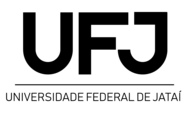
\includegraphics[width=1.5cm]{images/ufjJataiLogo.png}}

\begin{document}

	\begin{frame}
		\titlepage
	\end{frame}

	\AtBeginSection{
		\begin{frame}{Sum�rio}%[allowframebreaks]{Sum�rio}
    		\tableofcontents[currentsection]
    		%\tableofcontents[currentsection, hideothersubsections]
		\end{frame}
	}

	\begin{frame}{Plano de Aula}
		\tableofcontents
		%\tableofcontents[hideallsubsections]
	\end{frame}
	
	\section{Revis�o}

\begin{frame}{Problema}
\begin{block}{Problema 3.15 (a)}
	Mostre que a cole��o de linguagens decid�veis � fechada sob a opera��o de uni�o.		
\end{block} \pause
\begin{center}
	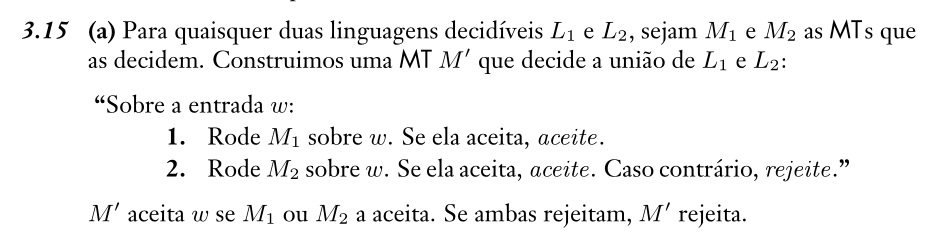
\includegraphics[height=2.7cm]{images/ex3-15a}
\end{center}
\end{frame}

\subsection{MT Multifita}
\begin{frame}[shrink]{MT Multifita}
\begin{block}{Defini��o}
Uma {\bf m�quina de Turing multifita} � como uma m�quina de Turing comum com v�rias fitas:
\begin{itemize} \pause
	\item cada fita tem sua pr�pria cabe�a de leitura e escrita; \pause
	\item a configura��o inicial consiste da cadeia de entrada aparecer sobre a fita 1, e as outras iniciar em branco; \pause
	\item a fun��o de transi��o permite ler, escrever e mover as cabe�as em algumas ou em todas as fitas simultaneamente
	\begin{center}
		$\delta : Q \times \Gamma^k \rightarrow Q \times \Gamma^k \times \{E,D,P\}^k$
	\end{center}
	em que $k$ � o n�mero de fitas.
\end{itemize}
\end{block}\pause
\begin{block}{Exemplo}
$\delta(q_i, a_1, \ldots, a_k) = (q_j, b_1, \ldots, b_k, P, D, \ldots, E)$
\end{block}
\end{frame}

\begin{frame}{MT Multifita}
\begin{block}{Teorema}
Toda m�quina de Turing multifita tem uma m�quina de Turing de uma �nica fita que lhe � equivalente.
\end{block}
\end{frame}

\section{Variantes da MT}

\begin{frame}{MT Multifita}
\begin{center}
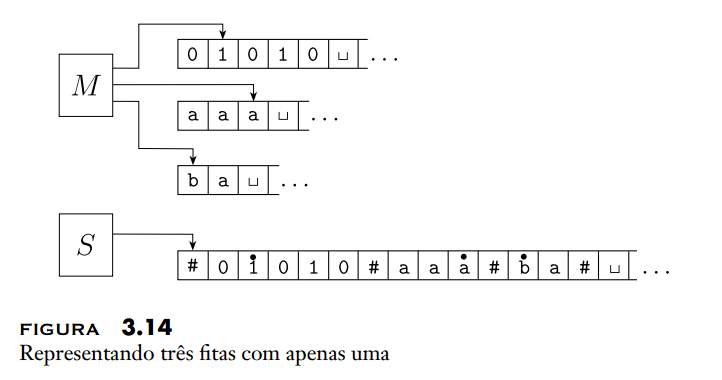
\includegraphics[height=6cm]{images/fig314.png}
\end{center}
\end{frame}

\begin{frame}{MT Multifita}
\begin{center}
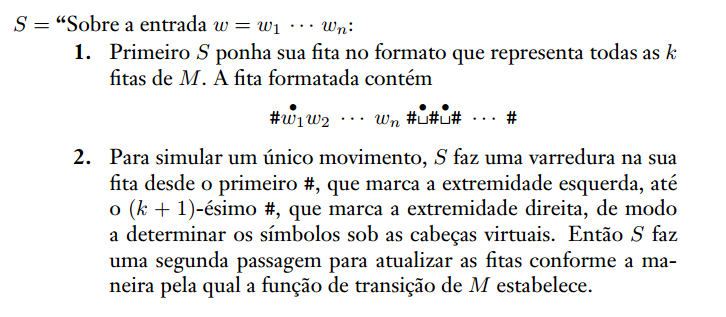
\includegraphics[height=5cm]{images/teoMt-1.png}
\end{center}
\end{frame}

\begin{frame}{MT Multifita}
\begin{center}
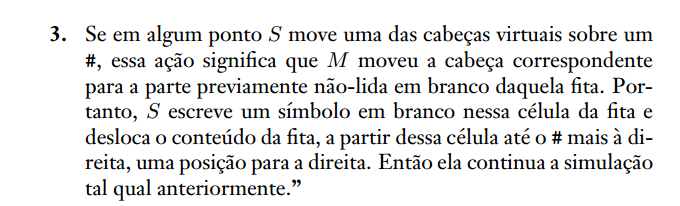
\includegraphics[height=3.3cm]{images/teoMt-2.png}
\end{center}
\end{frame}

\begin{frame}{MT Multifita}
\begin{block}{Teorema}
Toda m�quina de Turing multifita tem uma m�quina de Turing de uma �nica fita que lhe � equivalente.
\end{block} \pause
\begin{block}{Corol�rio}
Uma linguagem � Turing-reconhec�vel se e somente se alguma m�quina de Turing multifita a reconhece.
\end{block}
\end{frame}

\begin{frame}{MT Multifita}
\begin{center}
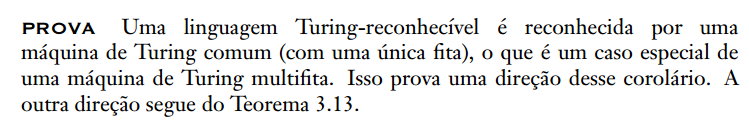
\includegraphics[height=1.8cm]{images/provaCorolario.png}
\end{center}
\end{frame}
	
	\begin{frame}
		\titlepage
	\end{frame}
	
\end{document}